\section{Introduction}

Personality is a comprehensive yet complex trait that encapsulates individual differences in patterns of thinking, feeling, and behaving~\cite{article}. Detecting personality automatically is of significant importance for improvement of machine's ability to have human-like cognition and engage in more natural interactions with humans, particularly in the context of advancing Artificial General Intelligence (AGI) and various practical applications such as reflective linguistic programming~\cite{fischer2023reflective}, disease diagnosis~\cite{6709853} and mental health prediction~\cite{feng2024far}. 
At the very beginning, owing to the limitations of multimedia model and computational power, researchers initially approached personality prediction as a straightforward text classification task, focusing on deciphering personality traits from individuals' digital footprints online~\cite{kerz2022pushing,yang_multi-document_2021}. However, as illustrated in Figure \ref{fig:example}, there is now growing recognition that personality is expressed across multiple modalities, with nuances that cannot be fully captured through text-based analysis alone~\cite{10.1145/3542954.3543012,ijcai2022p633,10030882}. This realization has driven the shift towards multimodal personality detection as the dominant methodology. Additionally, it is important to acknowledge that personality is not a static attribute for depicting behavior and emotions; rather, there is a novel concept called personality dynamics which refers to personality is not a fixed, unchanging set of traits but rather a fluid and evolving aspect of human psychology. This concept emphasizes that personality traits can shift over time due to various internal and external factors, including life experiences, environmental changes, and social interactions~\cite{9407599,doi:10.1177/08902070211022491}.
\begin{figure}[th]
  \centering
  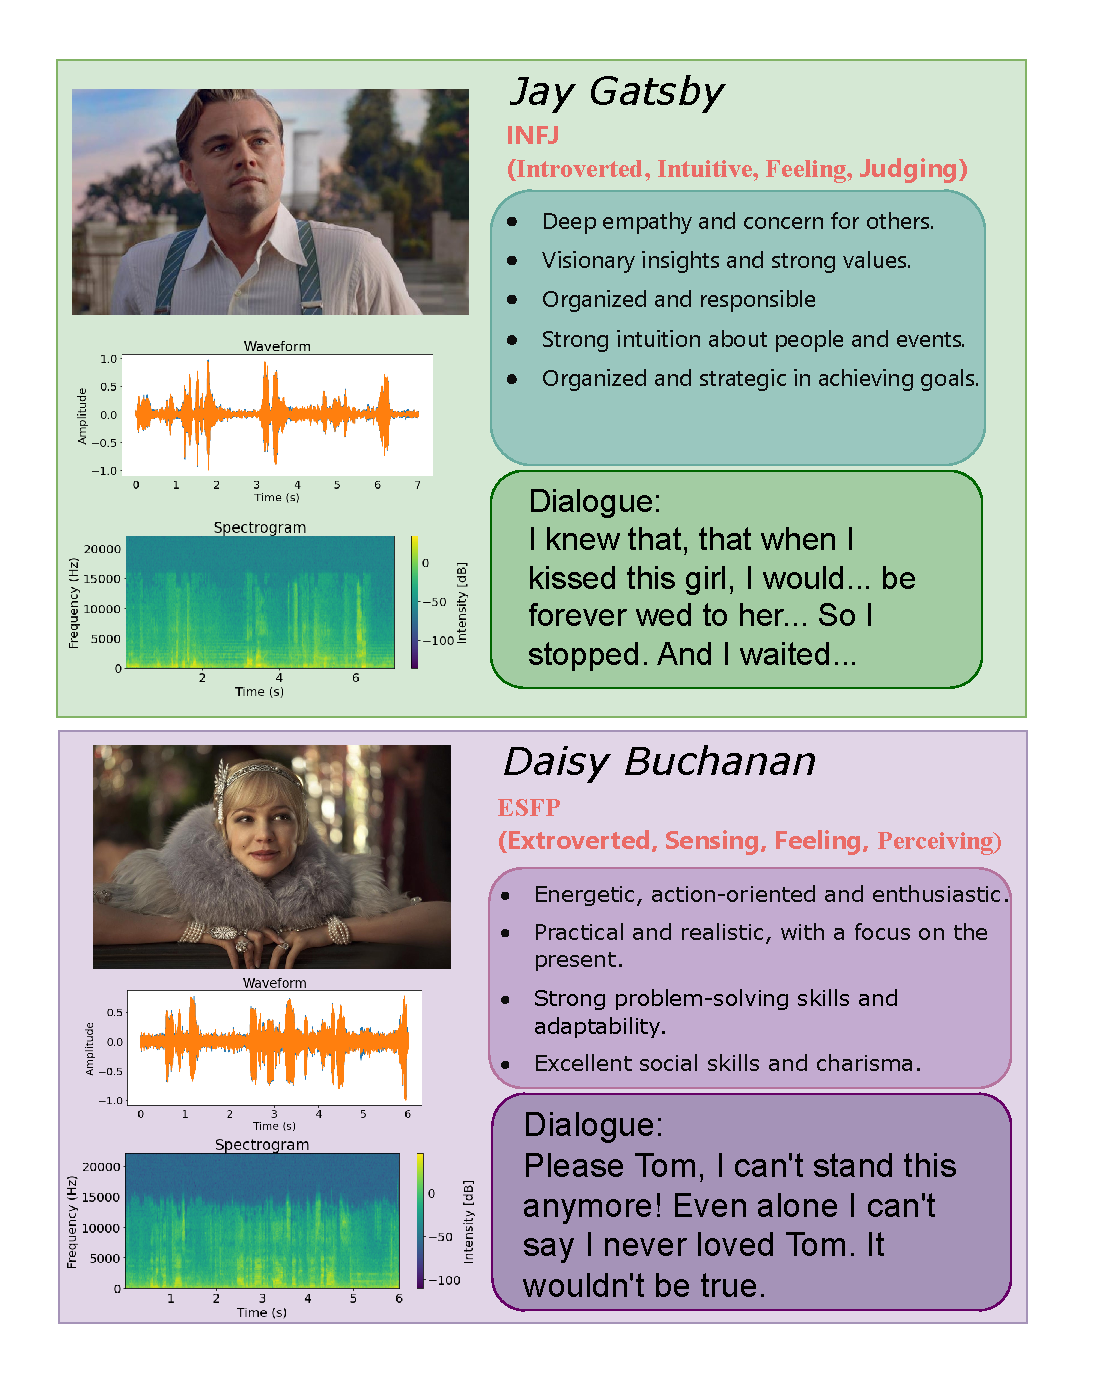
\includegraphics[width=\linewidth]{images/example.pdf}
  \caption{The Distinctive Features in Three Modalities for Personality Prediction}
  \label{fig:example}
\end{figure}

% \begin{figure}[ht]
%   \centering
%   % First subfigure
%   \begin{subfigure}[b]{\textwidth}
%       \centering
%       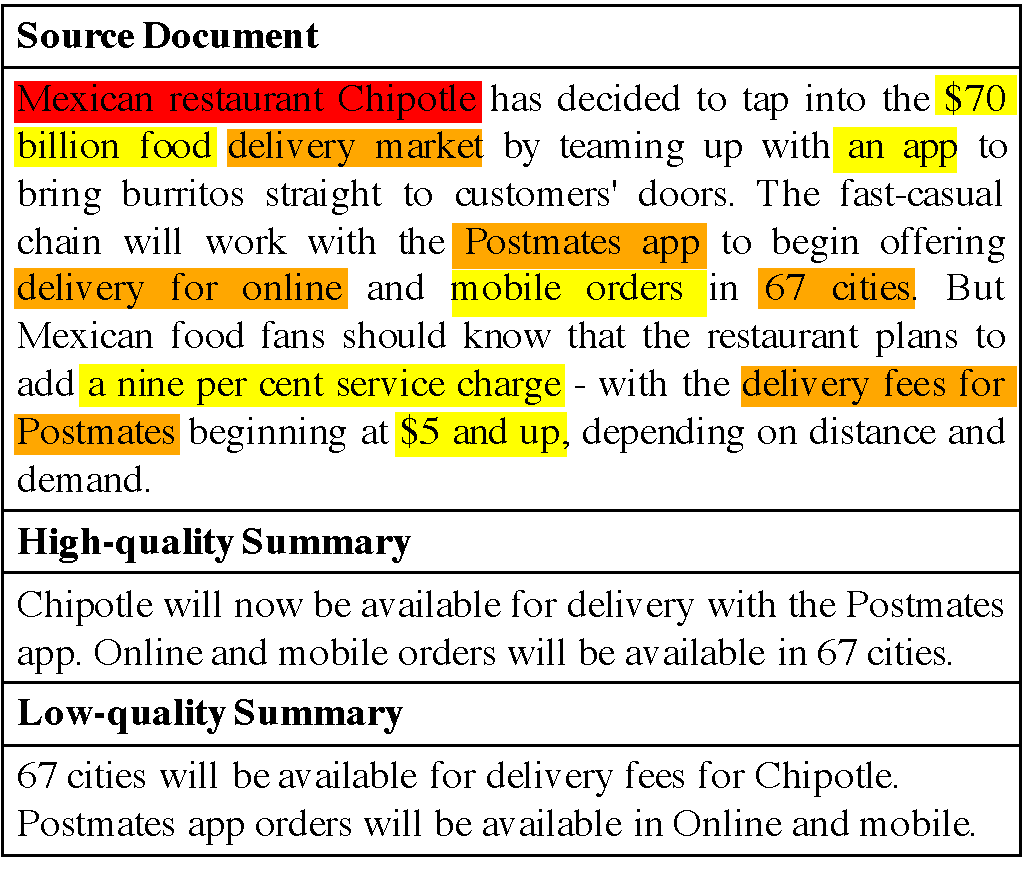
\includegraphics[width=\textwidth]{images/example1.pdf}
%       \label{fig:first}
%   \end{subfigure}
  
%   % Second subfigure
%   \begin{subfigure}[b]{\textwidth}
%       \centering
%       
\includegraphics[width=\textwidth]{images/example2.pdf}
%       \caption{Caption for second graph}
%       \label{fig:second}
%   \end{subfigure}
  
%   \caption{The Distinctive Features in Three Modalities for Personality Prediction}
%   \label{fig:combined}
% \end{figure}

Personality datasets, integrating text, audio, visual information along with the manner of speaking, face expressions, body language and so on, offer a richer, more nuanced view of human behavior and personality expressions than text-based datasets alone. This comprehensive approach is vital for developing models that accurately capture the complexity of human personality. Consequently, numerous multimodal datasets have been released in recent years, and several efforts have focused on constructing such datasets specifically for personality analysis~\cite{9407599,Junior_2021,Jiang_2020,chen2022cped}. Additionally, many multimodal datasets designed for other tasks have been adapted for personality prediction. For example, TVQA~\cite{Lei_2018}, a large-scale dataset originally created for visual question answering, is frequently utilized in personality research due to its extensive scope.

Although current datasets have evolved to include many features necessary for personality prediction, they still exhibit several limitations: 

1) \textbf{Limited Data Source}: Previous datasets often select one or several famous movies or TV series as the raw data, resulting in a limited number of characters and personality types covered, which hinders the generalizability of model training.

2) \textbf{Manual Annotation Issues}: The process of manually annotating personality traits typically relies on a few numbers of volunteers with varying levels of expertise, leading to potential inconsistencies and biases in the annotations.

3) \textbf{Lack of Dynamic Representation}: Current datasets largely fail to account for the dynamic nature of personality, which evolves over time in response to changes in life experiences and social environments. These datasets often provide static snapshots of personality traits, overlooking the psychological understanding that personality is fluid and can vary across different contexts and stages of life.


In our study, we endeavor to partially eliminate the aforementioned limitations by providing a scale-up multimodal dataset that contains reliable labels. Specifically, we find a personality database website\footnote[1]{https://www.personality-database.com/} that offers a large amount of personality types for virtual characters and \cite{zhu2023personalityaware} have scraped the personality data from it to annotate TVQA dataset. Compared with previous datasets whose labelling commonly involved five to ten people, our datasets are labelled by about 160 voters on average. It shows the vote distribution rather than a single personality type which is more persuasive and operable. As for the personality dynamics, we can analyze our dataset based on different relations and  Such networks provide a rich context for observing and understanding individual behaviors, preferences, and traits, reflecting the interconnectedness of personality with social and environmental factors.

Against these backdrops, we introduce the PersonaMovs, a comprehensive dataset that starkly contrasts with existing offerings in several key aspects. PersonaMovs is built on 305 movies and 14 TV series (894 episodes in total) in different genres, including more than \textbf{46k dialogues, 552k utterances, 4016 characters} and \textbf{963 hours videos}. With the rich annotation, our dataset supports 4 personality traits models (MBTI, Big Five, Enneagram and Instinctual Variant) with more 28 personality classes, 7 kinds of Social Relations and 8 attitudes for the Emotion Relations. Our analysis highlights substantial quantity and diversity in content, adequate experiments on different models with all modalities and personality dynamics discovery.

\begin{table*}[h]
  \centering
  \small
  \begin{tabular}{lllll}
    \hline
    \textbf{Dataset} & \textbf{Dialogues} & \textbf{Utters. / Dial} & \textbf{Characters} & \textbf{Source}\\
    \hline
    MEmoR & 8.53k & 64.23 & 7 & The Big Bang Theory \\
    \hline
    FriendsPersona & 0.71k & 27.61 & 7 & Friends\\
    \hline
    CPED & 12k & 1 & 392 & 40 TV shows\\
    \hline
    UDVIA & 188 & 65.31 & 147 & Dyadic Interaction\\
    \hline
    The ChaLearn FI & 10k & Unknown & 3000 & YouTube\\
    \hline
    TVQA & 29.4k & 2.2 & Unknown & 6 TV shows\\
    \hline
    \textbf{PersonaMovs} & 46.21k & 12.42 & 4000+ & 300+ Movies and 14 TV Shows\\
    \hline
  \end{tabular}
  \caption{Comparison of different datasets and our PersonaMovs}
  \label{tab:accents}
\end{table*}

Our contributions are as follows:
\begin{itemize}
  \item We introduce PersonaMovs, the most comprehensive and varied multimodal personality dataset to date, surpassing existing datasets in \textbf{scope} and \textbf{diversity}. This dataset uniquely combines movie and TV genres with personality analysis via audio, video, and text, along with crowdsourced personality, emotion, and social relations labels, unlocking new avenues in personality research\footnote[2]{\url{https://anonymous.4open.science/r/sample-of-MMPD-0177}}.
  \item We study seven model architectures from different model families. Our results show that PersonaMovs is more \textbf{difficult} compared to other datasets, not only because it has a larger amount of multimedia data, but also due to its diversity and similarity to real life. Through our analysis, we found that our dataset provides a more realistic reflection of the distribution of personalities in the real world, further enhancing its value for personality-related tasks.
  \item For the first time, we categorize 15 types of relations to depict the dynamics of character interactions on a scene-by-scene basis, enabling a granular analysis of personality \textbf{dynamics} through relations networks. Guided by the relations networks, we identify psychological phenomenons in both short-term and long-term conversational contexts, which largely explain the personality dynamics statistically. Personality as fluidity can be investigated  via our dataset, including fluidity across time as well as interpersonal relations
\end{itemize}



